\documentclass[]{book}
\usepackage{lmodern}
\usepackage{amssymb,amsmath}
\usepackage{ifxetex,ifluatex}
\usepackage{fixltx2e} % provides \textsubscript
\ifnum 0\ifxetex 1\fi\ifluatex 1\fi=0 % if pdftex
  \usepackage[T1]{fontenc}
  \usepackage[utf8]{inputenc}
\else % if luatex or xelatex
  \ifxetex
    \usepackage{mathspec}
  \else
    \usepackage{fontspec}
  \fi
  \defaultfontfeatures{Ligatures=TeX,Scale=MatchLowercase}
\fi
% use upquote if available, for straight quotes in verbatim environments
\IfFileExists{upquote.sty}{\usepackage{upquote}}{}
% use microtype if available
\IfFileExists{microtype.sty}{%
\usepackage{microtype}
\UseMicrotypeSet[protrusion]{basicmath} % disable protrusion for tt fonts
}{}
\usepackage{hyperref}
\hypersetup{unicode=true,
            pdftitle={Arabesque},
            pdfauthor={Gflowiz project team},
            pdfborder={0 0 0},
            breaklinks=true}
\urlstyle{same}  % don't use monospace font for urls
\usepackage{natbib}
\bibliographystyle{apalike}
\usepackage{longtable,booktabs}
\usepackage{graphicx,grffile}
\makeatletter
\def\maxwidth{\ifdim\Gin@nat@width>\linewidth\linewidth\else\Gin@nat@width\fi}
\def\maxheight{\ifdim\Gin@nat@height>\textheight\textheight\else\Gin@nat@height\fi}
\makeatother
% Scale images if necessary, so that they will not overflow the page
% margins by default, and it is still possible to overwrite the defaults
% using explicit options in \includegraphics[width, height, ...]{}
\setkeys{Gin}{width=\maxwidth,height=\maxheight,keepaspectratio}
\IfFileExists{parskip.sty}{%
\usepackage{parskip}
}{% else
\setlength{\parindent}{0pt}
\setlength{\parskip}{6pt plus 2pt minus 1pt}
}
\setlength{\emergencystretch}{3em}  % prevent overfull lines
\providecommand{\tightlist}{%
  \setlength{\itemsep}{0pt}\setlength{\parskip}{0pt}}
\setcounter{secnumdepth}{5}
% Redefines (sub)paragraphs to behave more like sections
\ifx\paragraph\undefined\else
\let\oldparagraph\paragraph
\renewcommand{\paragraph}[1]{\oldparagraph{#1}\mbox{}}
\fi
\ifx\subparagraph\undefined\else
\let\oldsubparagraph\subparagraph
\renewcommand{\subparagraph}[1]{\oldsubparagraph{#1}\mbox{}}
\fi

%%% Use protect on footnotes to avoid problems with footnotes in titles
\let\rmarkdownfootnote\footnote%
\def\footnote{\protect\rmarkdownfootnote}

%%% Change title format to be more compact
\usepackage{titling}

% Create subtitle command for use in maketitle
\providecommand{\subtitle}[1]{
  \posttitle{
    \begin{center}\large#1\end{center}
    }
}

\setlength{\droptitle}{-2em}

  \title{Arabesque}
    \pretitle{\vspace{\droptitle}\centering\huge}
  \posttitle{\par}
    \author{Gflowiz project team}
    \preauthor{\centering\large\emph}
  \postauthor{\par}
      \predate{\centering\large\emph}
  \postdate{\par}
    \date{2019-11-20}

\usepackage{booktabs}

\begin{document}
\maketitle

{
\setcounter{tocdepth}{1}
\tableofcontents
}
\hypertarget{about-arabesque}{%
\chapter{About Arabesque}\label{about-arabesque}}

Arabesque is a web application for thematic mapping of flow and networks datasets.
Built in javascript and HTML 5, it provides a full toolset to filter you data
and simplify it in order to make clearer and understandable maps.

This document aims to present the application and its fonctionnalities using
the provided datasets.

The documentation is segmented in several parts:

\begin{itemize}
\tightlist
\item
  \href{./main-page.html}{Main page}
\item
  \href{./functionnalities.html}{Main functionnalities}
\item
  \href{./import-a-dataset.html}{Import a dataset}
\end{itemize}

Please find the application at this address : \href{http://arabesque.ifsttar.fr/}{arabesque.ifsttar.fr} and more information on the project here : \href{https://geoflowiz.hypotheses.org/}{geoflowiz.hypotheses.org}.

Please report any issue on \href{https://github.com/gflowiz/arabesque}{GitHub}. This is a Free and OpenSource project, feel free to help us make it better.

\hypertarget{about-the-gflowiz-project}{%
\chapter{About the Gflowiz project}\label{about-the-gflowiz-project}}

Arabesque is part of the \href{https://geoflowiz.hypotheses.org/}{Gflowiz research project} on flow maps in the geoweb.

\hypertarget{main-page}{%
\chapter{Main page}\label{main-page}}

The main page welcomes you and provides several informations about the application
and a couple ways to enter it.

It is a page that you can scroll down. It is segmented in several parts:

\begin{itemize}
\tightlist
\item
  Welcome page
\item
  Documentation and demos
\item
  Gallery
\item
  General informations on the Gflowiz project
\item
  Detailed informations on the Arabesque application
\end{itemize}

\hypertarget{welcome-page}{%
\section{Welcome page}\label{welcome-page}}

\begin{figure}
\centering
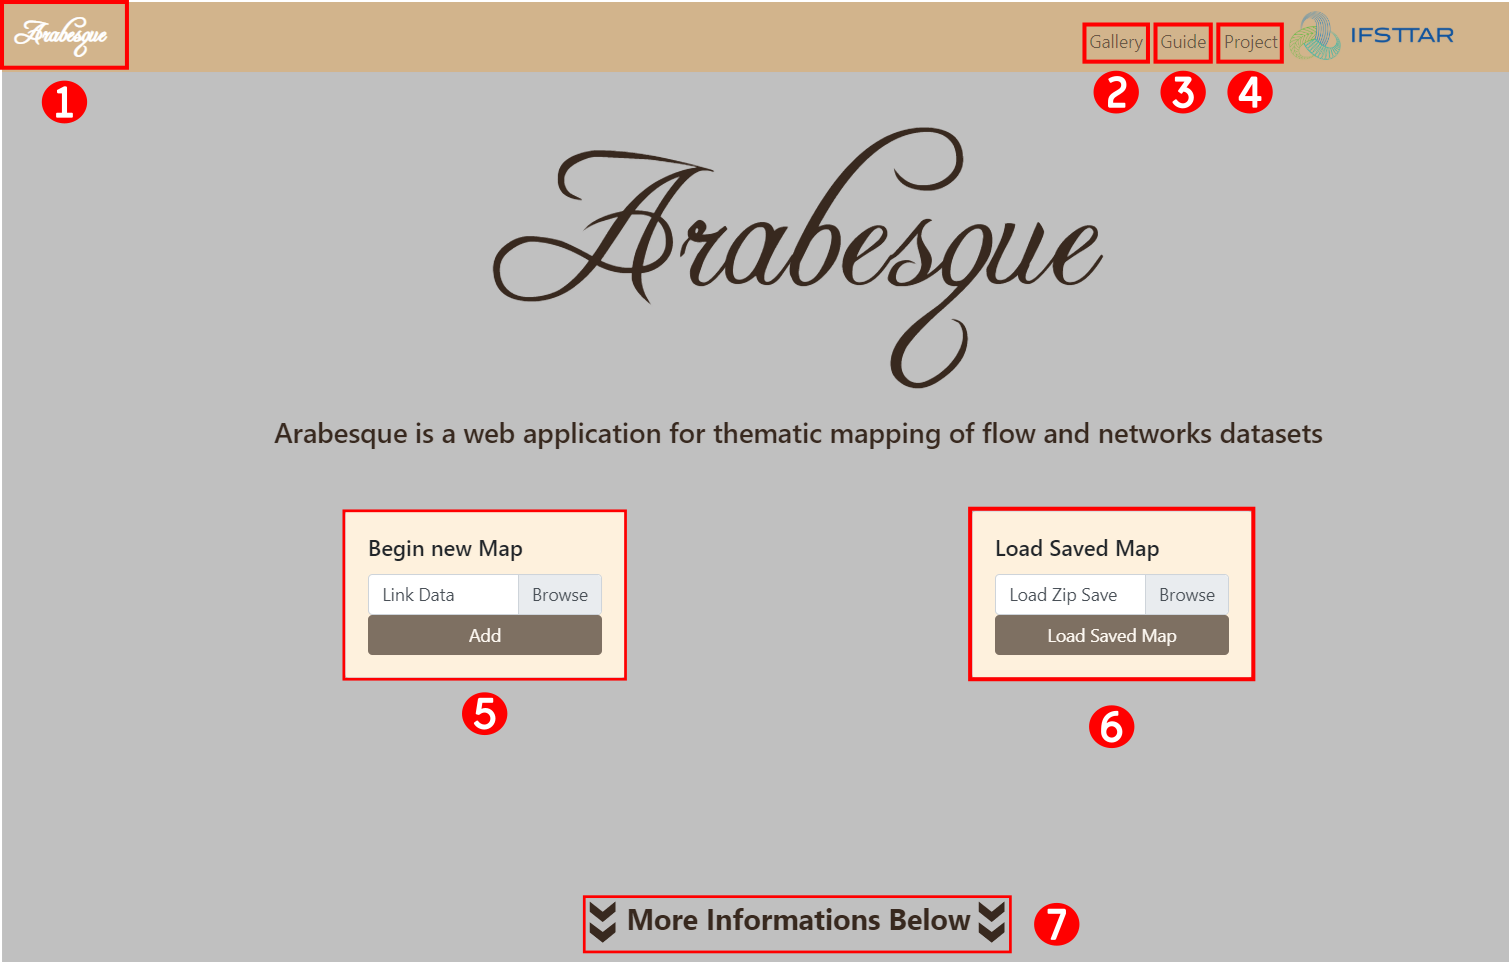
\includegraphics{images/main/01_arabesque_acceuil.png}
\caption{Welcome page}
\end{figure}

\begin{enumerate}
\def\labelenumi{\arabic{enumi}.}
\tightlist
\item
  Arabesque logo : click on it to return to the main page
\item
  Gallery button : to go directly to the gallery
\item
  Guide button : go to the guide
\item
  Project : visit the project website
\item
  New map : creating a new map with you own dataset
\item
  Load saved map : reload a map you created before
\item
  Scroll down to access more informations
\end{enumerate}

\hypertarget{documentation-and-demos}{%
\section{Documentation and demos}\label{documentation-and-demos}}

\begin{enumerate}
\def\labelenumi{\arabic{enumi}.}
\tightlist
\item
  You can come to this documentation by clicking on the link
\item
  Arabesque comes with 2 preloaded maps on several subjects:
\end{enumerate}

\begin{itemize}
\tightlist
\item
  London Bike Traffic
\item
  Swiss Migration
\end{itemize}

\begin{figure}
\centering
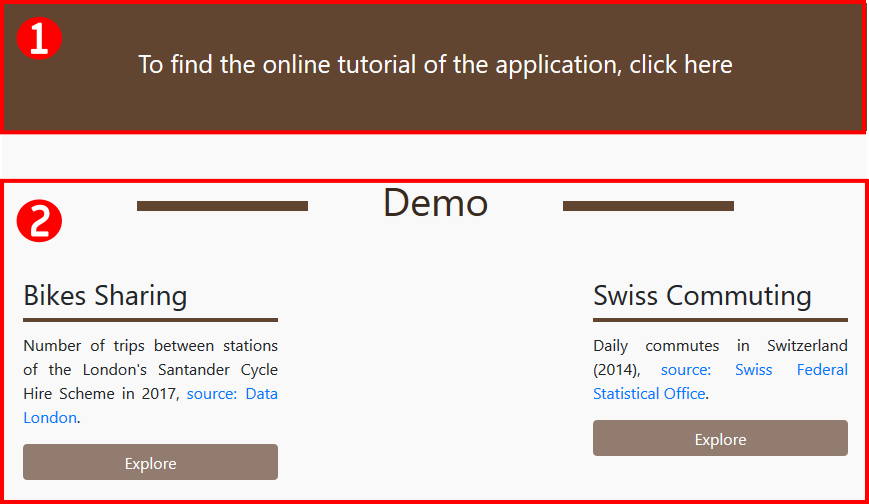
\includegraphics{images/main/03_arabesque_demos.png}
\caption{Demos}
\end{figure}

\hypertarget{gallery}{%
\section{Gallery}\label{gallery}}

A caroussel display several screenshots of maps realized with Arabesque.

\begin{figure}
\centering
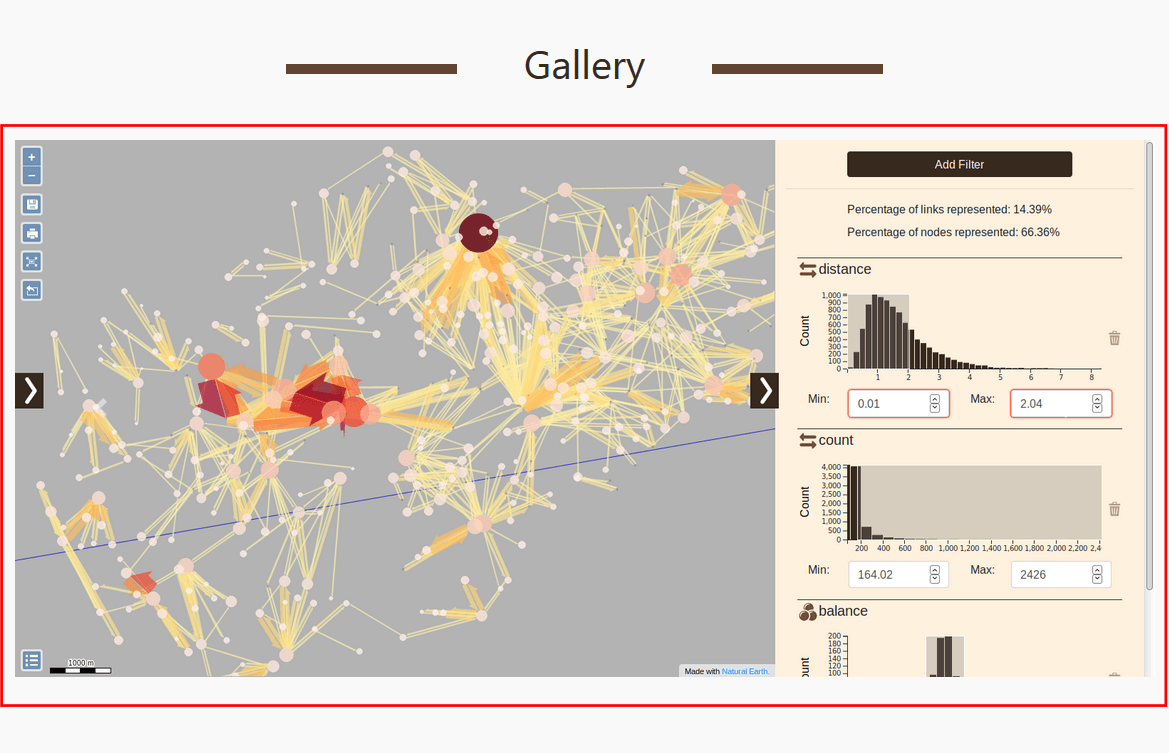
\includegraphics{images/main/02_arabesque_gallery.png}
\caption{Gallery}
\end{figure}

\hypertarget{general-informations}{%
\section{General informations}\label{general-informations}}

The main page provides general information on :

\begin{enumerate}
\def\labelenumi{\arabic{enumi}.}
\tightlist
\item
  the application (funding and
  contributors)
\item
  the Gflowiz project that Arabesque is part of.
\end{enumerate}

\begin{figure}
\centering
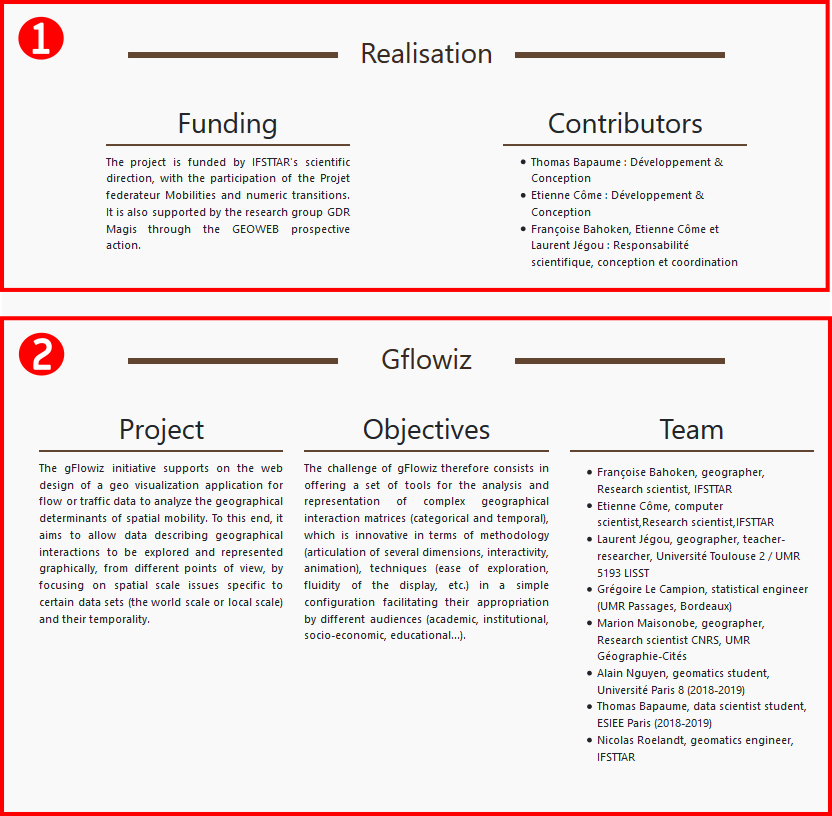
\includegraphics{images/main/05_arabesque_general_infos.png}
\caption{General informations}
\end{figure}

\hypertarget{detailed-informations}{%
\section{Detailed informations}\label{detailed-informations}}

Finally you can find detailled informations about the application :

\begin{itemize}
\tightlist
\item
  Software libraries
\item
  Source datasets
\item
  Licence
\item
  Link to the source code
\item
  Contact us policy
\end{itemize}

\begin{figure}
\centering
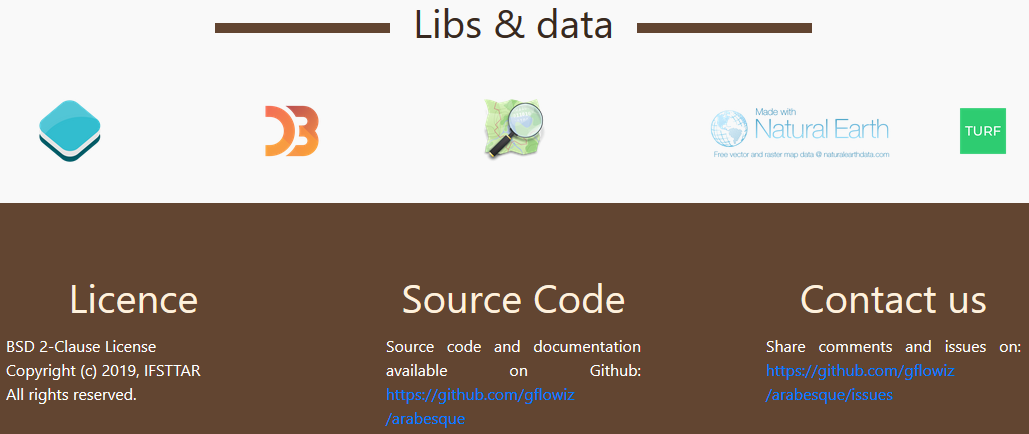
\includegraphics{images/main/06_arabesque_detailed_infos.png}
\caption{Detailed informations}
\end{figure}

\hypertarget{functionnalities}{%
\chapter{Functionnalities}\label{functionnalities}}

\hypertarget{launching-an-example}{%
\section{Launching an example}\label{launching-an-example}}

In order to test the differents functionnalities provided by Arabesque, we will use the Swiss communting demo.
Please find it in the Demo section and click on the \texttt{Explore} button (\texttt{1}).

\begin{figure}
\centering
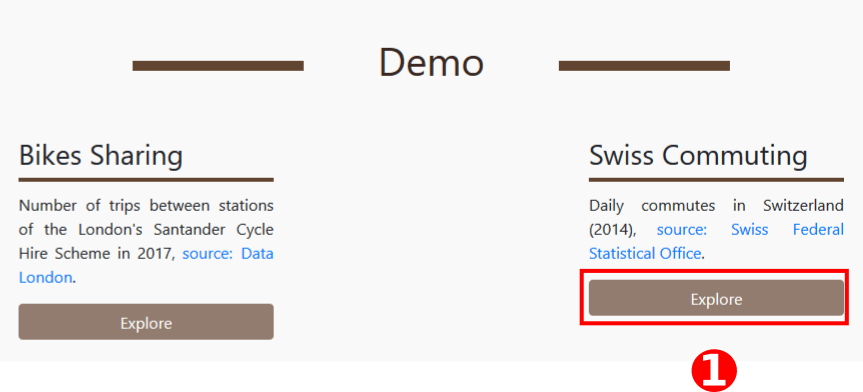
\includegraphics{images/functions/01_functions_launch_swiss_example.png}
\caption{Launching Swiss communting example}
\end{figure}

You might be greeted by a warning message. This is normal, if Arabesque find nodes
without links or links without nodes, it will remove them. It is based on a
join on nodes IDs.

\begin{figure}
\centering
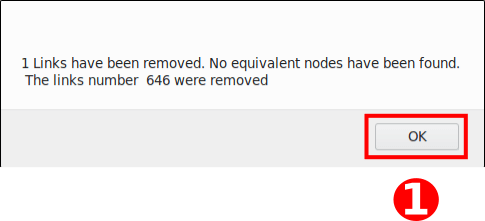
\includegraphics{images/functions/02_functions_swiss_example_warning.png}
\caption{Cleaning the dataset}
\end{figure}

\begin{enumerate}
\def\labelenumi{\arabic{enumi}.}
\tightlist
\item
  Click on \texttt{Ok}.
\end{enumerate}

\hypertarget{panels}{%
\section{Panels}\label{panels}}

Arabesque is divided in 3 panels:

\begin{enumerate}
\def\labelenumi{\arabic{enumi}.}
\tightlist
\item
  Layer management panel
\item
  Map panel
\item
  Data handling panel
\end{enumerate}

\begin{figure}
\centering
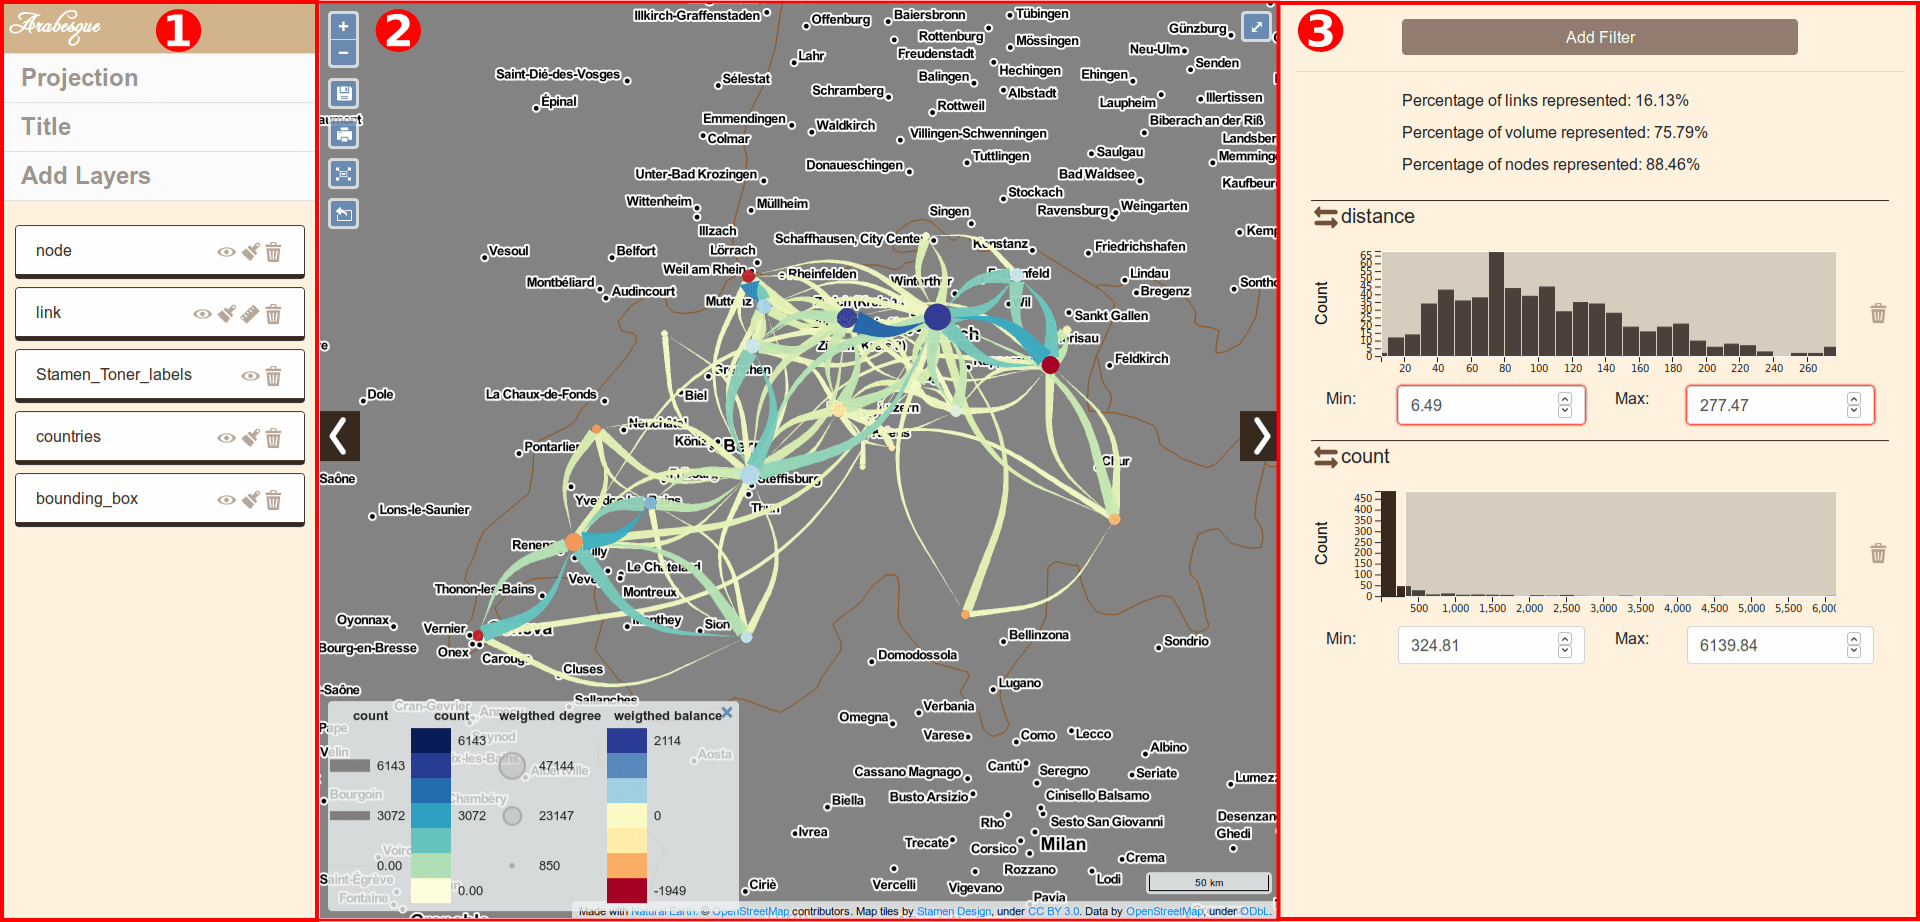
\includegraphics{images/functions/03_functions_swiss_example_main_window.png}
\caption{Arabesques panels}
\end{figure}

The side panels (layer and data) can be hidden by clicking on the arrows on the side. 
\includegraphics{images/functions/00_panels_arrow.png}

\hypertarget{layer-management-panel}{%
\subsection{Layer management panel}\label{layer-management-panel}}

The layer panel contains several buttons and tools to handle the layers.

\begin{figure}
\centering
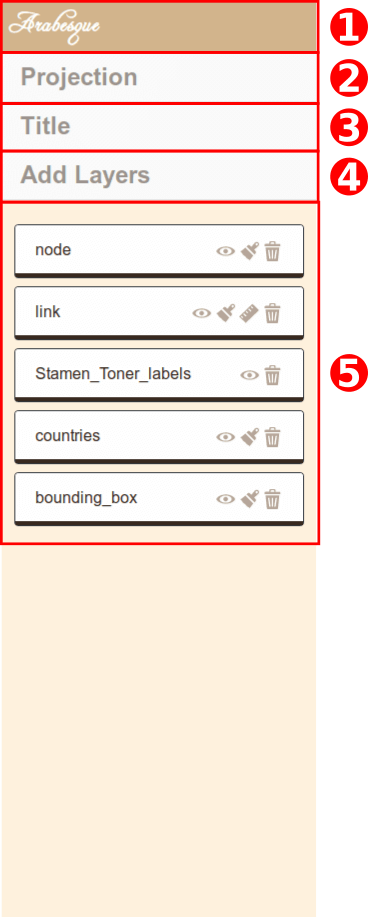
\includegraphics{images/functions/04_functions_swiss_example_layer_panel.png}
\caption{Arabesques panels}
\end{figure}

\begin{enumerate}
\def\labelenumi{\arabic{enumi}.}
\tightlist
\item
  Home button to get back to Welcome page
\item
  Projection : click to deploy the projection tool
\item
  Title : dialog box to change map title
\item
  Add layers: toolbox to add layers
\item
  Layers : area where you can manipulate the layer
\end{enumerate}

Let's see those how they work.

\hypertarget{projection-tool}{%
\subsubsection{Projection tool}\label{projection-tool}}

By default, entry data and project are into WGS84 (EPSG:4326), which is a Geographic Coordinnate system.
If it is great for dataset on a global scale, for more local ones, it might be
interesting to use \emph{projected coordinate system}.
Arabesque provides a series of preset projection but you can also provide an
EPSG code and the application will look for its definition on the website \href{https://epsg.io}{epsg.io}.

\begin{figure}
\centering
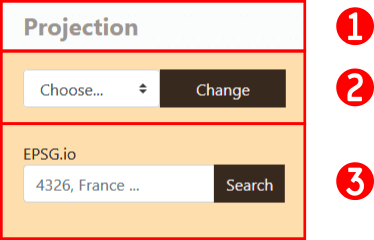
\includegraphics{images/functions/05_functions_swiss_example_projection_tool.png}
\caption{Projection toolbox}
\end{figure}

\begin{enumerate}
\def\labelenumi{\arabic{enumi}.}
\tightlist
\item
  Click on the \emph{Projection} button to deploy the toolbox
\item
  You can choose a projection from the list of provided ones
\item
  Or you can enter an EPSG code to get the definition from the web.
\end{enumerate}

\hypertarget{use-a-predefined-projection}{%
\paragraph{Use a predefined projection}\label{use-a-predefined-projection}}

\begin{figure}
\centering
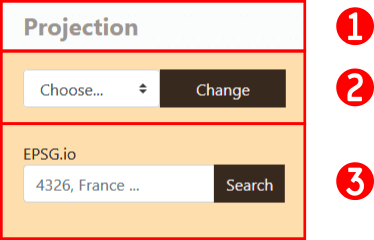
\includegraphics{images/functions/05_functions_swiss_example_projection_tool.png}
\caption{Projection toolbox}
\end{figure}

\begin{enumerate}
\def\labelenumi{\arabic{enumi}.}
\tightlist
\item
  Click on the button to deploy the drop-down list
\item
  Choose the projection you want
\item
  Click on \emph{Change} to change the map projection to the new one
\end{enumerate}

\begin{figure}
\centering
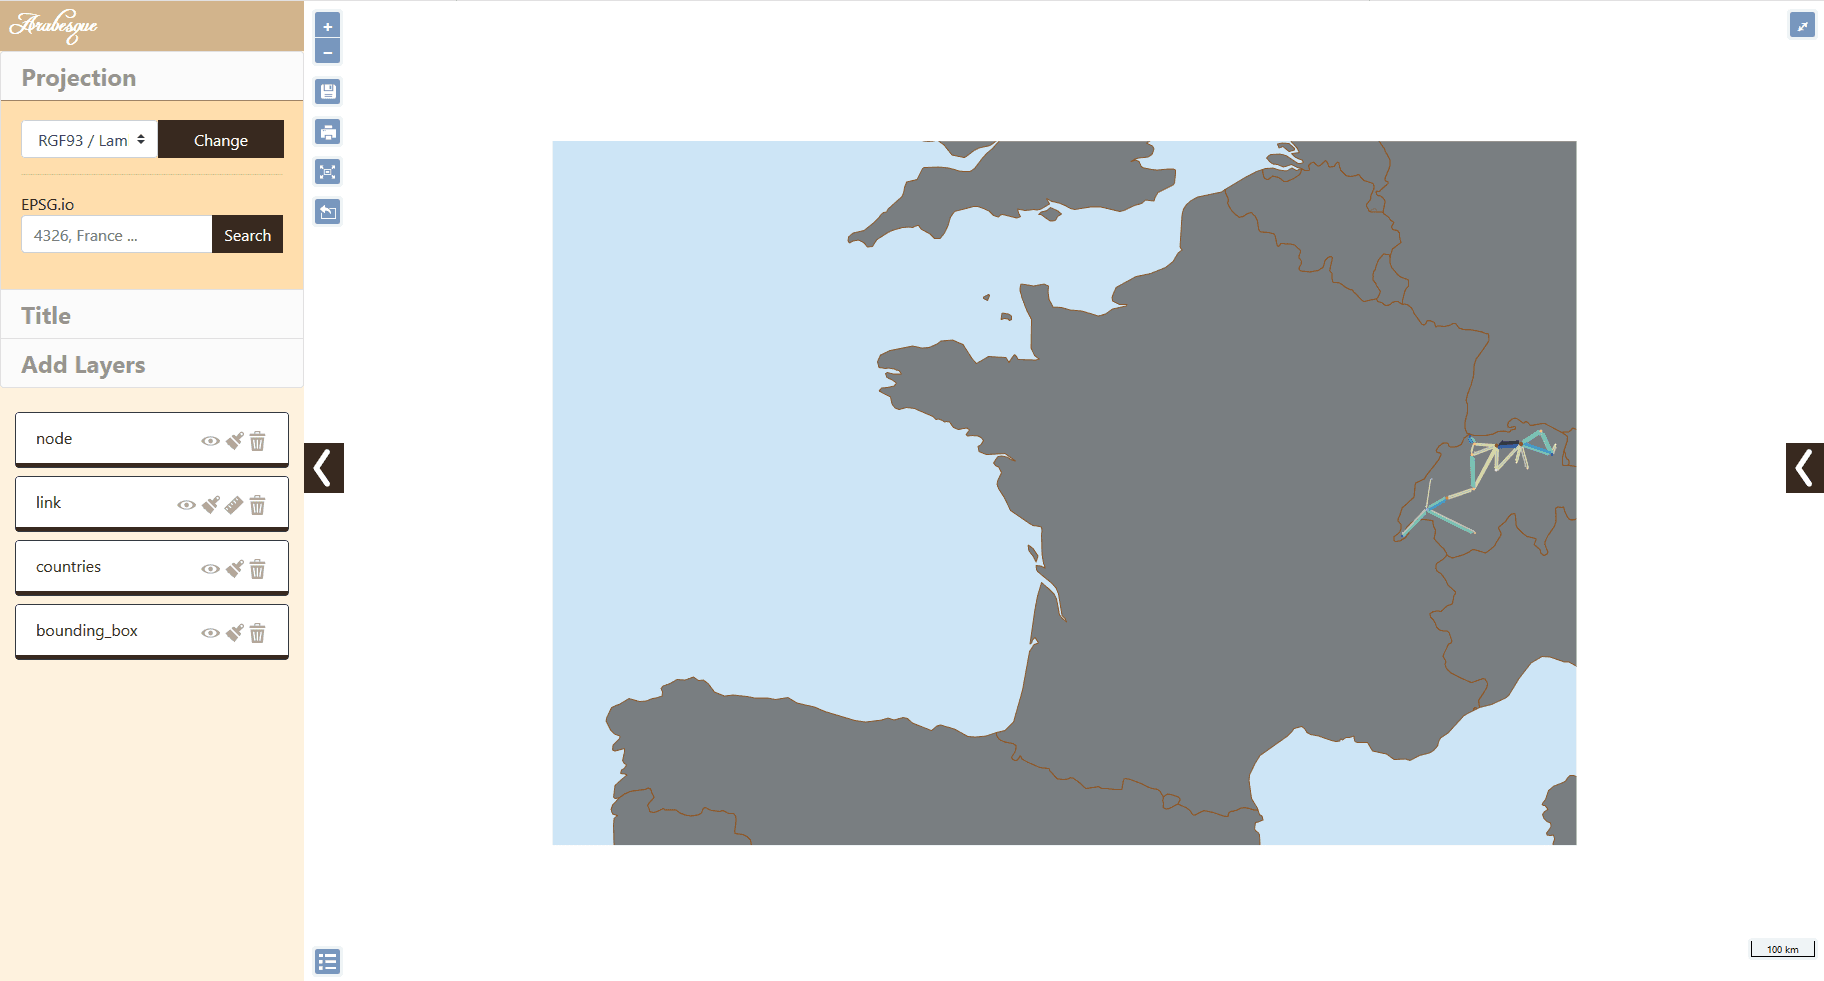
\includegraphics{images/functions/07_functions_swiss_example_projection_change.png}
\caption{Projection change}
\end{figure}

\hypertarget{map-panel}{%
\subsection{Map panel}\label{map-panel}}

\hypertarget{data-handling-panel}{%
\subsection{Data handling panel}\label{data-handling-panel}}

\hypertarget{import-a-dataset}{%
\chapter{Import a dataset}\label{import-a-dataset}}

In this part, we will show you how to import a dataset into the application.

\bibliography{book.bib}


\end{document}
